\subsection{Overview}
In this whole chapter the architecture design process is described, and it contains all the significant
architecture decisions. 
Therefore, first of all, in this section a high-level and very general architecture for the TrackMe 
project is presented and discussed.  

\begin{figure}[H]
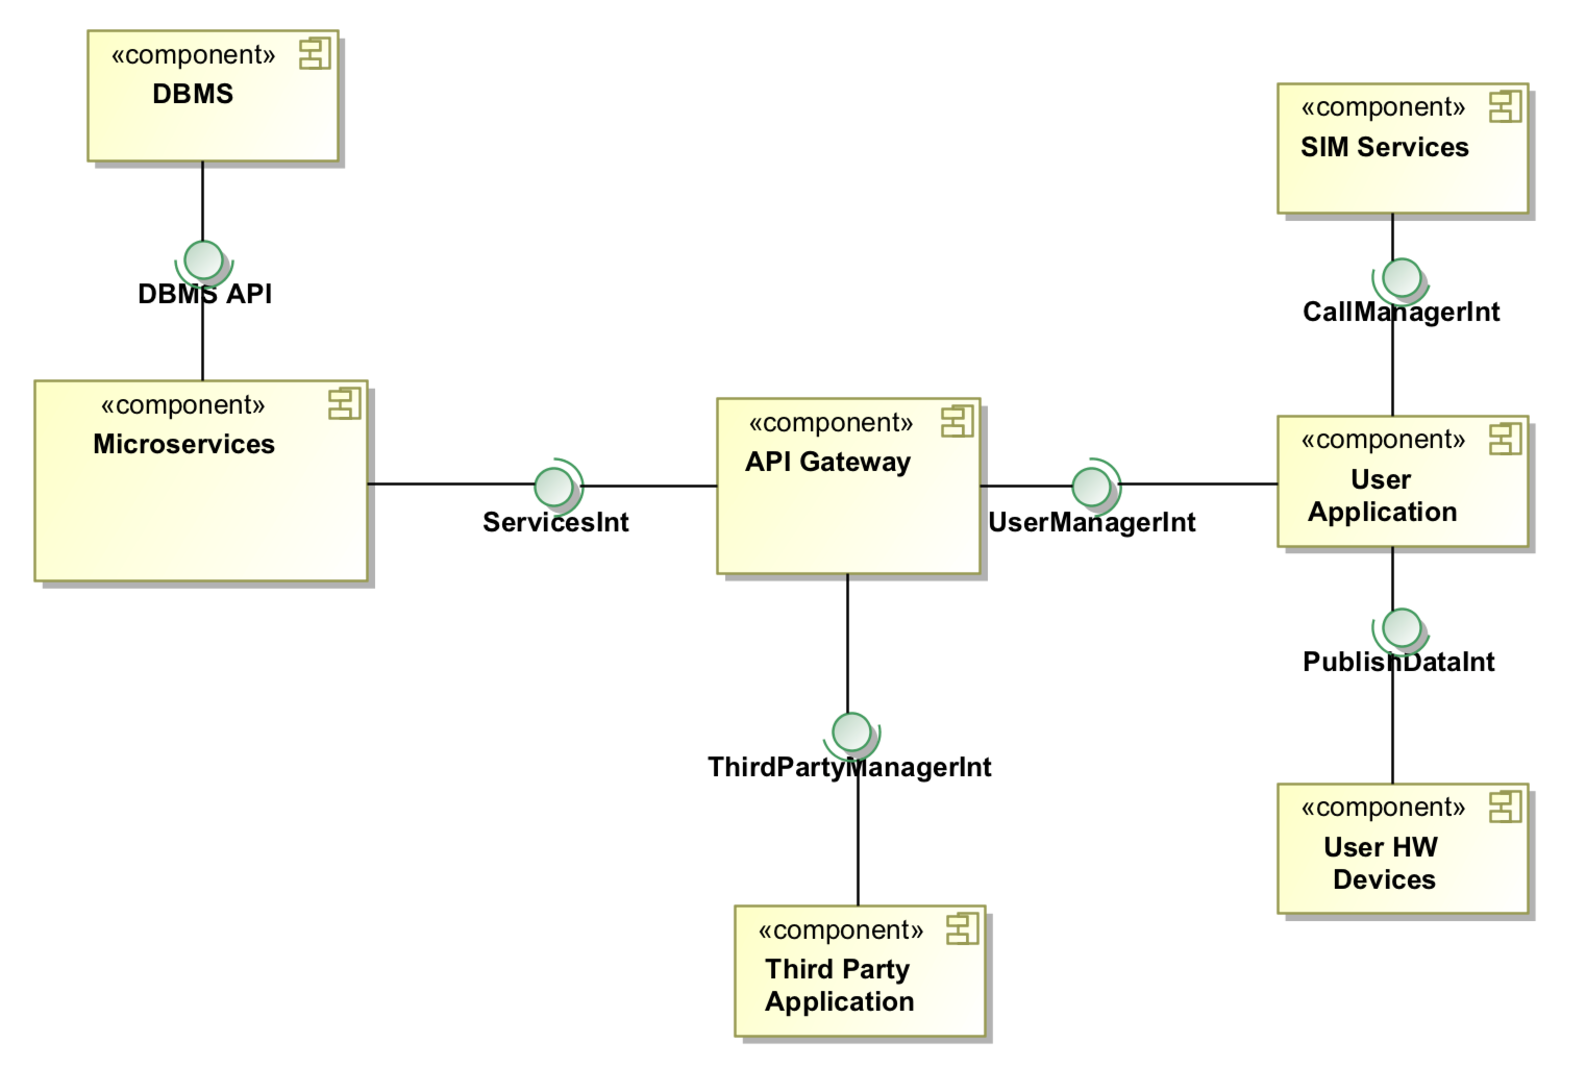
\includegraphics[width=\linewidth]{Images/highlevelcd.pdf}
\caption{ High-level component diagram }
\label{fig:highlevelcomponentdiagram}
\end{figure}

As a reference architecture, the microservices one has been considered: this decision will be later discussed. \\
From the picture, it is evident that the clients can access the services by means of an API gateway, that will provide authentication 
to the users, and forwards the requests to the correct microservices based on the service registry.
Of course, a new service instance needs to register to the service registry in order to be located by the API gateway. \\
Another relevant information is that the project can be ideally split, at a high level, into two applications: one for the users and one for the third parties customers: they both interact with the API gateway, that will guarantee to access all the
microservices that compose the core functionality of the business.
More specifically, the "microservices" block includes Data4Help and Track4Run functions, while the goals
of AutomatedSOS service are reached locally and directly by means of the user application, that, when
needed, will perform a call with the help of the SIM service. 
The user application also needs to communicate with a device that is able to collect data regarding his health: more specifically, this
instrument will send data toward the user application autonomously, without being asked.
Examples of  this machines are smartrings and smartwatches. 
The data regarding the position of the user is, instead, retrieved via GPS's API. \\
Note, also, that the microservices need to keep some data persistent, and, thus access to a DBMS, by means
of its API. 
Moreover, some services need also to communicate and share information: this is achieved via the message queue, that is
charged of receiving and forwarding messages to the interested parts. \\

